%%%%%%%%%%%%%%%%%%%%%%%%%%%%%%%%%%%%%%%%%%%%%%%%%%%%%%%%%%%%%%%%%%%%%%%%%%%%%%%%
%
%   Basic configuration
%
%%%%%%%%%%%%%%%%%%%%%%%%%%%%%%%%%%%%%%%%%%%%%%%%%%%%%%%%%%%%%%%%%%%%%%%%%%%%%%%%

% Use 'KOMA-Script Book' as the document class
\documentclass[toc=bibliography,toc=indentunnumbered]{scrbook} 

% All modern documents should start with this (unless you use XeTeX/LuaTeX)
\usepackage[utf8]{inputenc}      % UTF-8 file encoding
\usepackage[T1]{fontenc}         % 8-bit font encoding

% This package is useful for modding standard environments
\usepackage{etoolbox}



%%%%%%%%%%%%%%%%%%%%%%%%%%%%%%%%%%%%%%%%%%%%%%%%%%%%%%%%%%%%%%%%%%%%%%%%%%%%%%%%
%
%   Page design
%
%%%%%%%%%%%%%%%%%%%%%%%%%%%%%%%%%%%%%%%%%%%%%%%%%%%%%%%%%%%%%%%%%%%%%%%%%%%%%%%%

% Font size
\KOMAoptions{fontsize=11pt}

% Line spacing
\linespread{1.05}

% Paper format
\KOMAoptions{paper=B5}

% Duplex layout
\KOMAoptions{twoside}

% Page layout (ISO B5 aspect ratio)
%\KOMAoptions{BCOR=6mm}
%\KOMAoptions{DIV=11}

% Page layout (Golden aspect ratio)
\areaset[6mm]{358.40pt}{579.89pt} 

% Disable headers
\pagestyle{plain}

% Page numbers
\addtokomafont{pagenumber}{\vspace{3.5ex}\footnotesize\sffamily\bfseries}

% Left-justify equations
\PassOptionsToPackage{fleqn}{amsmath}

% Use spacing instead of indentation to separate paragraphs
%\KOMAoptions{parskip=half+} 



%%%%%%%%%%%%%%%%%%%%%%%%%%%%%%%%%%%%%%%%%%%%%%%%%%%%%%%%%%%%%%%%%%%%%%%%%%%%%%%%
%
%   Document fonts
%
%%%%%%%%%%%%%%%%%%%%%%%%%%%%%%%%%%%%%%%%%%%%%%%%%%%%%%%%%%%%%%%%%%%%%%%%%%%%%%%%

% Palatino serif font (main text font)
\usepackage[largesc]{newpxtext}

% Kepler serif font (main text font)
%\usepackage{kpfonts}

% Optima sans font (titles, captions, footnotes, and links)
%\usepackage{classico}

% Biolinum sans font (titles, captions, footnotes, and links)
\usepackage[scaled=1.07]{biolinum}

% Euler mathematical font (math)
\usepackage[utf8]{eulerpx/eulerpx}

% Vera monospaced font (code)
\usepackage[scaled=0.84]{beramono}

% Enable microtypographic tweaks
\usepackage{microtype}


 
%%%%%%%%%%%%%%%%%%%%%%%%%%%%%%%%%%%%%%%%%%%%%%%%%%%%%%%%%%%%%%%%%%%%%%%%%%%%%%%%
%
%   Table of contents
%
%%%%%%%%%%%%%%%%%%%%%%%%%%%%%%%%%%%%%%%%%%%%%%%%%%%%%%%%%%%%%%%%%%%%%%%%%%%%%%%%
 
% Load a package for styling the table of contents
\usepackage{tocstyle}

% Place page numbers right after the section entries
\usetocstyle{nopagecolumn}

% Do not include subsections in the table of contents
\setcounter{tocdepth}{1}

% Use tabular lining figures for the sections, but oldstyle figures for the pages
\settocstylefeature{entryhook}{\tlfstyle}
\settocstylefeature{pagenumberhook}{\osfstyle}
\settocstylefeature[0]{entryhook}{\tlfstyle\bfseries}
\settocstylefeature[0]{pagenumberhook}{\osfstyle\bfseries}



%%%%%%%%%%%%%%%%%%%%%%%%%%%%%%%%%%%%%%%%%%%%%%%%%%%%%%%%%%%%%%%%%%%%%%%%%%%%%%%%
%
%   Headings
%
%%%%%%%%%%%%%%%%%%%%%%%%%%%%%%%%%%%%%%%%%%%%%%%%%%%%%%%%%%%%%%%%%%%%%%%%%%%%%%%%

% Make sure all headings use sans text and math
\addtokomafont{disposition}{\sffamily}

% Change the sizes of chapters and sections
\addtokomafont{chapter}{\huge}
\addtokomafont{section}{\large}

% Change spacing around chapters and sections
\RedeclareSectionCommand[beforeskip=-0.0\baselineskip,afterskip=0.7\baselineskip]{chapter}
\RedeclareSectionCommand[beforeskip=-1.0\baselineskip,afterskip=0.5\baselineskip]{section}

% Bringhurst-style chapter numbers
\makeatletter
\newsavebox{\feline@chapter}
\newcommand\feline@chapter@marker[1][4cm]{\sbox\feline@chapter{\resizebox{!}{#1}{\setlength{\fboxsep}{0pt}\colorbox{white}{\color{gray}\thechapter}}}\usebox{\feline@chapter}}
\renewcommand*{\chapterformat}{\sbox\feline@chapter{\feline@chapter@marker[1.6cm]}\makebox[0pt][l]{\makebox[\dimexpr\textwidth+\marginparsep+\wd\feline@chapter\relax][r]{\usebox\feline@chapter}}}
\makeatother

% Hanging chapter titles
\renewcommand*{\chapterheadstartvskip}{\hspace*{-1.5\parindent}}



%%%%%%%%%%%%%%%%%%%%%%%%%%%%%%%%%%%%%%%%%%%%%%%%%%%%%%%%%%%%%%%%%%%%%%%%%%%%%%%%
%
%   Captions
%
%%%%%%%%%%%%%%%%%%%%%%%%%%%%%%%%%%%%%%%%%%%%%%%%%%%%%%%%%%%%%%%%%%%%%%%%%%%%%%%%

% Switch to a sans font for captions
\addtokomafont{caption}{\sffamily\small}

% Use a bold font for caption labels
\addtokomafont{captionlabel}{\sffamily\bfseries\small}

% Redefine the caption label delimiter
%\renewcommand*{\captionformat}{\hspace{0.3em}\rule[-0.30ex]{0.085em}{1.80ex}\hspace{0.3em}}

% Add 2em margins on each side of the caption. (Since the default \parindent is 1em, this
% implies that the left end of the caption will always look one \parindent indented if it
% comes right before/after a new paragraph, and can therefore prevent weird indentation.)
\setcapdynwidth{\dimexpr\textwidth-4em\relax}

% Disable extra indentation of the subsequent lines in a multiline caption
\setcapindent{0em}



%%%%%%%%%%%%%%%%%%%%%%%%%%%%%%%%%%%%%%%%%%%%%%%%%%%%%%%%%%%%%%%%%%%%%%%%%%%%%%%%
%
%   Footnotes
%
%%%%%%%%%%%%%%%%%%%%%%%%%%%%%%%%%%%%%%%%%%%%%%%%%%%%%%%%%%%%%%%%%%%%%%%%%%%%%%%%

% Make sure footnote marks are separated by commas and kerned properly
\usepackage{fnpct}

% Switch to a sans font for footnotes
\addtokomafont{footnote}{\sffamily}

% Change footnote marks to letters (recommended if using superscript citations)
%\renewcommand{\thefootnote}{\alph{footnote}}

% Set the footnote rule length to the text width
\setfootnoterule{\textwidth}

% Disable the footnote rule entirely
%\setfootnoterule{0pt}

% Adjust the footnote size and spacing
\deffootnote{1em}{1em}{\textsuperscript{\thefootnotemark}\kern0.1em}



%%%%%%%%%%%%%%%%%%%%%%%%%%%%%%%%%%%%%%%%%%%%%%%%%%%%%%%%%%%%%%%%%%%%%%%%%%%%%%%%
%
%   Hyperlinks
%
%%%%%%%%%%%%%%%%%%%%%%%%%%%%%%%%%%%%%%%%%%%%%%%%%%%%%%%%%%%%%%%%%%%%%%%%%%%%%%%%

% Enable clickable hyperlinks (useful if the document is read on a computer)
\usepackage{hyperref}

% Do not color links (suitable for documents that will primarily be printed)
\hypersetup{hidelinks}

% Generate links in the table of contents
\hypersetup{linktoc=all}

% Generate links to footnotes
\hypersetup{hyperfootnotes}

% Generate PDF bookmarks (also useful if the document is read on a computer)
\hypersetup{bookmarks,bookmarksopen,bookmarksnumbered}

% Switch to a sans font for hyperlinks
\urlstyle{sf}

% Fix kerning problems for backslashes and redefine underscores in hyperlinks
\makeatletter
\let\UrlSpecialsOld\UrlSpecials
\def\UrlSpecials{\UrlSpecialsOld\do\/{\Url@slash}\do\_{\Url@underscore}}%
\def\Url@slash{\@ifnextchar/{\kern+0.05em\mathchar47\kern-0.10em}%
    {\kern0.08em\mathchar47\penalty\UrlBigBreakPenalty}}
\def\Url@underscore{\nfss@text{\leavevmode \kern.06em\vbox{\hrule height 0.12ex width 0.4em}}}
\makeatother




%%%%%%%%%%%%%%%%%%%%%%%%%%%%%%%%%%%%%%%%%%%%%%%%%%%%%%%%%%%%%%%%%%%%%%%%%%%%%%%%
%
%   References
%
%%%%%%%%%%%%%%%%%%%%%%%%%%%%%%%%%%%%%%%%%%%%%%%%%%%%%%%%%%%%%%%%%%%%%%%%%%%%%%%%

% Bibliography backend (e.g. 'biber' or 'bibtex')
\PassOptionsToPackage{backend=biber}{biblatex}

% Bibliography style (e.g. 'nature' or 'numeric-comp')
\PassOptionsToPackage{style=nature}{biblatex}

% Citation style (e.g. 'plain' or 'superscript')
\PassOptionsToPackage{autocite=plain}{biblatex}

% Format for cross-references with \cref
\PassOptionsToPackage{noabbrev}{cleveref}
\newcommand{\crefrangeconjunction}{--}



%%%%%%%%%%%%%%%%%%%%%%%%%%%%%%%%%%%%%%%%%%%%%%%%%%%%%%%%%%%%%%%%%%%%%%%%%%%%%%%%
%
%   Load packages
%
%%%%%%%%%%%%%%%%%%%%%%%%%%%%%%%%%%%%%%%%%%%%%%%%%%%%%%%%%%%%%%%%%%%%%%%%%%%%%%%%

% Load the required packages
\usepackage{amsmath}    % Common mathematical environments
\usepackage{biblatex}   % Produces the bibliography
\usepackage{cleveref}   % Easy and consistent cross-references
\usepackage{graphicx}   % Loads and displays figures
\usepackage{booktabs}   % Proper formatting of tables
\usepackage{siunitx}    % Proper formatting of units
\usepackage{mhchem}     % Proper formatting of chemicals
\usepackage{lipsum}     % Filler text



%%%%%%%%%%%%%%%%%%%%%%%%%%%%%%%%%%%%%%%%%%%%%%%%%%%%%%%%%%%%%%%%%%%%%%%%%%%%%%%%
%
%   Miscellaneous
%
%%%%%%%%%%%%%%%%%%%%%%%%%%%%%%%%%%%%%%%%%%%%%%%%%%%%%%%%%%%%%%%%%%%%%%%%%%%%%%%%

% Set tables in a sans font
\AtBeginEnvironment{tabular}{\sffamily}
\AtBeginEnvironment{tabular*}{\sffamily}

% Format for typesetting physical units
\sisetup{range-units=single}
\sisetup{range-phrase=--}
\sisetup{detect-all} 

% Use 2em equation indentation
\makeatletter
\setlength\@mathmargin{2em}
\makeatother

% Replace \cite with the more flexible \autocite
\let\cite=\autocite



%%%%%%%%%%%%%%%%%%%%%%%%%%%%%%%%%%%%%%%%%%%%%%%%%%%%%%%%%%%%%%%%%%%%%%%%%%%%%%%%
%
%   Document itself
%
%%%%%%%%%%%%%%%%%%%%%%%%%%%%%%%%%%%%%%%%%%%%%%%%%%%%%%%%%%%%%%%%%%%%%%%%%%%%%%%%

\addbibresource{library.bib}

\begin{document}

\frontmatter
\tableofcontents
\chapter*{Abstract}\noindent
This is a \textsc{latex} template intended for academic theses, and was put together by \href{https://github.com/jabirali}{Jabir Ali Ouassou} while preparing his PhD dissertation.
The template itself is released under a Creative Commons Attribution licence (\href{https://creativecommons.org/licenses/by/4.0/}{\textsc{cc by 4.0}}).
This basically means that you are free to use the template for any purpose as long as you give appropriate credit.

The template bundles the \href{https://github.com/libertinus-fonts/libertinus}{Libertinus fonts}, which is used for all regular text and mathematics, and the \href{https://ctan.org/tex-archive/fonts/urw/classico}{\textsc{urw} classico} fonts, which are used for chapter and section headings.
The former is available under the Open Font Licence (\textsc{sil ofl 1.1}), and is free for both private and commercial use.
The latter is available under the Aladdin Free Public Licence (\textsc{afpl}), and is only free for non-commercial use.
If commercial use is of importance, a suitable replacement for \textsc{urw} classico would be the Libertinus Sans fonts, which are also bundled with the template.

Note that this template relies on \textsc{lualatex} for \eg font customization, and on \textsc{bibtex} for reference handling.
For command-line users, the easiest way to compile the document is to run \texttt{latexmk -lualatex thesis.tex}.
If using an \textsc{ide}, please check the program settings for how to enable compilation with \textsc{lualatex} and \textsc{bibtex}.
The template is based on the \textsc{koma-script} book class (\texttt{scrbook}), so for further customization of the template, please check out \href{https://ctan.org/pkg/koma-script}{their documentation}.

The template does not include a title page.
This is because the style requirements typically varies between universities, and many institutions will anyway autogenerate a titlepage upon thesis submission.

\chapter*{Preface}\noindent
\lipsum


\mainmatter 
\chapter{Introduction}
Blah.
 
\chapter{Quasiclassical theory}
In here: define notation, propagators, and matrix current.
Make it clear what approximations we have performed.

\section{Propagators}
\section{Matrix current}
%Usadel diffusion equation:
%\begin{equation}
%  iD \nabla\cdot\mathbf{I} = U 
%\end{equation}
%Boundary conditions:
%\begin{equation}
%  \mathbf{I}_a = \mathbf{I}_b = [g_a, g_b]
%\end{equation}

\section{Novel notation}
Regarding the notation... How about simply saying fuck special notation for spin and nambu space? I mean, the reason we're having problems with overnotation is:
\begin{itemize}
  \item 2×2 matrices in spin space has underline-notation;
  \item 2×2 matrices in nambu space has hat-notation;
  \item 4×4 matrices in spin-nambu space has underline+hat notation;
  \item 8-element vectors in our rho-space has vec notation;
  \item The resulting 8×4×4 basis vector $\rho$ should get vec+underline+hat notation;
  \item We haven't chosen a notation for 8×8 matrices in rho-space yet...
\end{itemize}
And so on. It becomes chaos, and at this point, all the extra notation will rather serve to confuse the reader than help the reader grok what we're doing. Also,
the more special notation of this kind, the larger the risk of mistakes -- and a single mistake in all of these hats and underlines will cause a lot of confusion for the reader.

So how about this: we drop as much annotation as possible, and just use explicit definitions instead, like explicitly saying "we define the 8-element vector..." or "define the 8×8 matrix" etc instead of implying this from notation.

First of all, fuck non-quasiclassical quantities. All our equations are quasiclassical anyway, so we might as well not reserve e.g. $\check{G}$ for the non-quasiclassical propagator. 
So we define the Green's function etc as:
\begin{align}
\bm{G} &= \begin{bmatrix}\bm{G}^R & \bm{G}^K \\ 0 & \bm{G}^A \end{bmatrix}, &
\bm{J} &= \begin{bmatrix}\bm{J}^R & \bm{J}^K \\ 0 & \bm{J}^A \end{bmatrix}, &
\bm{U} &= \begin{bmatrix}\bm{U}^R & \bm{U}^K \\ 0 & \bm{U}^A \end{bmatrix}.
\end{align}
No underline, no check, no hat. Just bold letters, with a superscript that mentions R/K/A as usual.
Then we use lower-case letters for the spin-space decomposition:
\begin{align}
\bm{G}^R &= \begin{bmatrix}+\bm{g}^R & +\bm{f}^R \\ -\tilde{\bm{f}}^R & -\tilde{\bm{f}}^R \end{bmatrix}, &
\bm{J}^R &= \begin{bmatrix}+\bm{j}^R & +\bm{i}^R \\ -\tilde{\bm{i}}^R & -\tilde{\bm{j}}^R \end{bmatrix}, &
\bm{U}^R &= \begin{bmatrix}+\bm{u}^R & +\bm{v}^R \\ -\tilde{\bm{v}}^R & -\tilde{\bm{u}}^R \end{bmatrix}. &
\end{align}
When we define these, we explicitly say that all the lower-case quantities are 2×2 matrices in spin-space.
Then we explicitly define the rhos as:
\begin{align*}
  \bm\rho_0 &= \text{diag}(+\bm\sigma_0, +\bm\sigma_0^*), &
  \bm\rho_4 &= \text{diag}(+\bm\sigma_0, -\bm\sigma_0^*), \\
         &\;\;\vdots                             &
         &\;\;\vdots                             \\
  \bm\rho_3 &= \text{diag}(+\bm\sigma_3, +\bm\sigma_3^*), &
  \bm\rho_7 &= \text{diag}(+\bm\sigma_3, -\bm\sigma_3^*), \\
\end{align*}
where we mention that $\sigma_0$ is the identity and $\sigma_n$ the 2×2 Pauli matrices.
Then we say that we group these into an 8-element vector:
\begin{equation}
  \vec{\bm\rho} = [\bm\rho_0, \ldots, \bm\rho_7]
\end{equation}
At this point, we introduce a single new notation: things with a vector arrow have a structure in the 8-dimension spin-nambu vector space defined here.
We then define the new notation for the distribution function and currents in this new space:
\begin{align}
  \bm{H} &= \vec{H} \cdot \vec{\bm{\rho}}, &
  \bm{J} &= \vec{J} \cdot \vec{\bm{\rho}}.
\end{align}
So we dot two vector quantities, namely the 8-element vector and the 8×4×4-element basis vector, and get a 4×4-element matrix out.
No bold for the 8-element vectors, as they're in a different space.
I'm using a capital letter for the distribution function to follow the implicit ``lower-case letters are spin-space'' logic.
The inverse transformation is:
\begin{align}
  \vec{H} &= \text{Tr}[ \bm{H} \vec{\bm{\rho}} ] / 4, &
  \vec{J} &= \text{Tr}[ \bm{J} \vec{\bm{\rho}} ] / 4
\end{align}
So we "trace away" the matrix structure to map the distribution function onto our 8-element vector space.
Once we have two 8-element vector quantities, we define an 8×8 relationship between them using tensor notation:
\begin{align}
  \vec{J} = \tensor{M} \vec{H}
\end{align}
 
\chapter{Algorithms}

\cleardoublepage
\section*{Steffensen's method with linear mixing}
The selfconsistent solution for the superconducting gap~$Δ$ can be expressed
\[
  Δ = f(Δ),
\]
where the mean field $Δ = Δ(\B{r})$ in general is a function of position, and the function evaluation $f(Δ)$ implies solving both the Usadel equation and selfconsistency equation for the gap.
This fixpoint equation can be rewritten\\[-2ex]
\[
  d(Δ) \deq f(Δ) - Δ = 0,
\]
where the function $d(Δ)$ quantifies the difference after one fixpoint iteration for a gap~$Δ$.
This can be solved more efficiently using \eg Newton's method,
\[
  Δ_{n+1} = Δ_n - \frac{d(Δ_n)}{d'(Δ_n)}.
\]
In general, we do not know the exact form of $d'(Δ_n)$, so it has to be estimated numerically. 
For this, we may use a forward difference approximation,
\[
  d'(Δ_n) \approx \frac{d(Δ_{n+1}) - d(Δ_n)}{Δ_{n+1} - Δ_n},
\]
so that the Steffensen equation for convergence acceleration can be written
\[
  Δ_{n+3} = Δ_n - \frac{d(Δ_n)(Δ_{n+1} - Δ_n) }{d(Δ_{n+1}) - d(Δ_{n})}.
  \label{eq:steffensen}
\]
In the special case that we use regular fixpoint iterations between Steffensen boosts, we simply have $d(Δ_n) = Δ_{n+1} - Δ_n$, so this equation simplifies to
\[
  Δ_{n+3} = Δ_n - \frac{(Δ_{n+1} - Δ_n)^2 }{Δ_{n+2} - 2Δ_{n+1} + Δ_n} .
\]
Another alternative is to use \emph{linear mixing}.
We then perform fixpoint iterations as usual, but restrain the changes using a mixing factor~$α\in[0,1]$:\\[-2ex]
\[
  Δ_{n+1} = αf(Δ_n) + (1-α)Δ_n 
\]
Note that using an iteration pattern like this, $d(Δ_n) = Δ_{n+1} - Δ_n$ does not hold anymore.
However, by solving the equation above for $f(Δ_n) - Δ_n$, we just find that the corresponding expression just has an extra factor~$1/α$:
\[
  d(Δ_n) \deq f(Δ_n) - Δ_n = [Δ_{n+1} - Δ_n]/α.
\]
Going back to \cref{eq:steffensen}, we see that since there is only one factor~$d(\,\cdot\,)$ in the numerator and one in the denominator, the resulting factors~$α$ cancel out, leading to the same Steffensen iteration equation as before.

\clearpage


\section{Critical temperature calculations}
\section{Steffensen's method}

\clearpage
\section{Interpolation}
When solving the nonequilibrium problem, the problem was formulated as:
\begin{align}
  \begin{pmatrix}
    \BC{H}\phantom{'} \\
    \BC{H}' 
  \end{pmatrix}'
  =
  -
  \begin{pmatrix}
    \B{0} & 
    \B{1} \\
    \BC{M}^{-1} \big[ (\partial_z\BC{M}) + \BC{Q} \big] &
    \BC{M}^{-1} \big[ (\partial_z\BC{Q}) + \BC{K} \big]
  \end{pmatrix}
  \begin{pmatrix}
    \BC{H}\phantom{'} \\
    \BC{H}' 
  \end{pmatrix}
\end{align}
One nice thing about this formulation, is that we have an explicit expression for the Jacobian $\B{J}$ of the problem, i.e. the $16\times16$ proportionality matrix in the equation above, which does not depend on the distribution function~$\BC{H}$.

However, each of the matrices $\BC{M}$, $\BC{Q}$, $\BC{K}$ are functions of the equilibrium propagators $\U{G}^R$ and $\U{G}^A$, which again depend on position~$z$.
This means that the Jacobian~$J(z)$ is position-dependent, and can only be explicitly calculated at the discretized positions where the equilibrium propagators are known.
The problem is that the differential equation solver needs to be able to calculate the Jacobian at arbitrary positions, which means that some form of interpolation is needed here.
My first approach was a simple linear interpolation.
That was unstable and crashed, since the numerical solver is sensitive to the \emph{derivative} of the Jacobian, which in this case becomes discontinuous.
My next approach was to try using the \texttt{pchip}-library (Piecewise Hermitian Cubic Interpolation) that I've used for cubic interpolations of e.g. the gap in the past.
However, this library only operates on scalar functions, and calling it $16^2 = 256$ separate times to interpolate the Jacobian at each point turned out to be really inefficient.
My solution was therefore to implement such a cubic matrix interpolator myself, in order to speed up the nonequilibrium solver.

\clearpage
\section{Kinetic equation}
As we have shown before...



\clearpage
\section{Boundary condition}
As we showed in the manuscript with Tom [Eq.~(31--32)], the boundary conditions at a spin-active interface can be written as follows:
\begin{align}
  \BC{J}_a &= \BC{C}_{aa} \BC{H}_a - \BC{C}_{ab} \BC{H}_b \\
  \BC{J}_b &= \BC{C}_{bb} \BC{H}_b - \BC{C}_{ba} \BC{H}_a 
\end{align}
The minus-sign on the right-hand sides appears because this is derived from a commutator. 
This sign is just a convenient convention -- in comparison to Tom's notation, this gets rid of the signs in Eq.~(36) of the arXiv manuscript.
Note that both the boundary conditions above follow the same pattern:
\begin{align}
  \BC{J} &= \BC{C} \BC{H} - \BC{C}'\BC{H}'
\end{align}
Here, the unprimed quantities refer to ``this'' side of the interface -- i.e. where the current $\BC{J}$ is calculated -- while the primed ones refer to ``the other'' side.

If we for now ignore spin-orbit coupling, we can substitute $\BC{J} = \BC{M}\partial\BC{H} + \BC{QH}$ into the equation above, and thus get the boundary condition:
\begin{align}
  \BC{M}\partial\BC{H} + \BC{QH} = \BC{C} \BC{H} - \BC{C}'\BC{H}'
\end{align}
This is equivalent to Eq.~(40) in the arXiv manuscript, but fixes a sign error in the $\BC{Q}$-term. 
This boundary condition can also be written in matrix form:
\begin{align}
  \BC{M}\partial\BC{H} + [\BC{Q}-\BC{C}]\BC{H} + \BC{C}'\BC{H}' = 0
\end{align}
Finally, this can be rewritten in matrix form as:
\begin{align}
  \begin{pmatrix}
    \BC{Q}-\BC{C} & \BC{M} \\
  \end{pmatrix}
  \begin{pmatrix}
    \BC{H} \\
    \partial\BC{H}
  \end{pmatrix}
  +
  \begin{pmatrix}
    \BC{C}' & 0 \\
  \end{pmatrix}
  \begin{pmatrix}
    \BC{H} \\
    \partial\BC{H}
  \end{pmatrix}
  &= 0
\end{align}
In other words: if we define the 16-element state vectors $\B{u} = [\BC{H}; \partial\BC{H}]$ and $\B{u}\ = [\BC{H}'; \partial\BC{H}']$, and the $8\times16$ matrices $\B{A} = [\BC{Q}-\BC{C}, \BC{M} ]$ and $\B{B} = [-\BC{C}', 0]$ that operate on these, then the boundary condition can be written:
\begin{align}
  \B{A}\B{u} - \B{B}\B{u}' = 0 .
\end{align}
\clearpage
These boundary conditions have a number of nice properties:
\begin{itemize}
  \item 
    The coefficients $\B{A}$ and $\B{B}$ only depend on equilibrium properties.
    This means that they only have to be calculated once, and evaluating the boundary condition is reduced to a simple matrix multiplication.
  \item 
    The equation has the form $\B{F}(\B{u},\B{u}') = 0$.
    This is perfect since I use a numerical solver that works by minimizing a user-specified residual.
  \item
    The Jacobian $J_{ij} = \partial F_i/\partial u_j$ of the boundary condition is simply the matrix $\B{A}$.
    Since I use a numerical solver that can use the Jacobian of the boundary condition to speed up convergence, this is quite useful.
\end{itemize}
In the case of transparent boundary conditions, the problem may again be formulated in the same way as above, but with Jacobians $\B{A} = \B{B} = [\B{1},\B{0}]$.
 
\chapter{Introduction and motivation}
In this chapter, we investigate how LaTeX renders random mathematical expressions and cross-references that we throw at it.
Furthermore, we evaluate how adequate \textsc{otf} fonts are for mathematical publishing.
Finally, this is used to ascertain whether \textsc{\oldstylenums{stix2}} is suitable for thesis writing.

The chapter starts with a test of mathematical expressions in \cref{sec:test}, and continues with a \emph{Lorem Ipsum} citation in \cref{sec:test2}.
Both sections include tests related to cross-references, figures and tables.



\clearpage
\section{Here be random text about \textsc{srt/lrt}}\label{sec:test}
This is a test. Let's see how this goes! Btw, $e^{i\pi} = -1$ and $(\partial_\mu \partial^\mu - m^2) \psi = 0$.
Also calligraphic $\mathcal{A} = \mathcal{F}x$.
Bold $\symbf{A}\symbf{\xi} = \symbf{\eta}$ and spins $f_{\uparrow\downarrow}+g_{\downarrow\uparrow} \in \mathbb{S}_{\parallel\perp}$ and $n\in\mathbb{N}$.
Also $\partial_z I = \partial_z \Delta = 0$.
Also, we know well that $I(\varphi) = I_0 \sin \varphi$.  And also $\mathbf{R}\mathbb{R} \otimes \mathbf{C}\mathbb{C} \oplus \mathbf{N}\mathbb{N}_+$.\footnote{This is simply just a simple test, with an equation $\sin a = \cos(2b-1)/\cos(2b+1)$. And here is a chemical element \ce{CrO23} and physical unit \SI{12e3}{m}. }%\footnote{Testing}\footnote{Testing again}\footnote{Test}\footnote{Test}\footnote{Test}\footnote{Test}\footnote{Test}\footnote{Test}\footnote{Test}
%Also we can point out $I = \{ 1 \pm [\sin(a)\tan(b)]^2\} $.
Here is another equation:
%\begin{equation}
%  Δ(z) = \int_0^{ω_c} \mathrm{d}ε\;\mathrm{Re}\; f_s(ε) \tanh\!\left(\frac{π}{2e^γ} \frac{ε/Δ_0}{T/T_c}\right)
%\end{equation}
\begin{equation}
  \Delta(z) = \int_0^{\infty} \mathrm{d}\epsilon\,\mathrm{Re}\, f_s(\epsilon) \tanh\!\left(\frac{\pi}{2e^\gamma} \frac{\epsilon/\Delta_0}{T/T_c}\right)
\end{equation}
Some references are given in \cref{ch:test}, and more specifically \cref{sec:test,sec:test2}.
\begin{equation}
  \int f(x) dx \sum_i n_i \prod_j p_j
\end{equation}
Here is some normal text. \textit{And here is some emphasized text 1234567890}. Normal 123456789. 
Say something about the \textsc{bcs} theory and \textsc{bcs-bec} transition \emph{and \textsc{srt/lrt} in italics}.
This is another test: $1 < 2 > 0 \leq 1 \geq 2$, and here is an url: \url{http://www.google.com/interesting_something/else/and/even/more/stuff}
%\verb+for i=[0:0.1:1.0] do f(i,j) = 1/g(j,i)+
\begin{equation}
  \textit{e}e\mathrm{e}\textsf{e}%\texttt{e}\;
  \textit{I}I\mathrm{I}\textsf{I}%\texttt{I}\;
  \textit{m}m\mathrm{m}\textsf{m}%\texttt{m}
\end{equation}
\textsf{And here is some sans-serif text with math $e^{i\varphi}=\cos\varphi+i\sin\varphi$ and so on.} And here is some normal text again.
Here is a chemical equation \ce{CrO23} and unit \SI{23e23}{m/s} but $J_0 = \SI{23e23}{m/s}$ also.

%\subsection{Miscellaneous symbols}
%\begin{equation}
%\mathbf{ABCDEFGHIJKLMOPQRSTUVWXYZ}
%\end{equation} 
%\begin{equation}
%\mathbf{abcdefghijklmnopqrstuvwxyz}
%\end{equation} 
%\begin{equation}
%ABCDEFGHIJKLMOPQRSTUVWXYZ
%\end{equation} 
%\begin{equation}
%abcdefghijklmopqrstuvwxyz
%\end{equation} 
%\begin{equation}
%\alpha\beta\gamma\delta\varepsilon\theta\vartheta\phi\varphi\psi\eta\kappa\lambda
%\end{equation} 
%\begin{equation}
%\Gamma\Delta\Theta\Phi\Psi\Lambda
%\end{equation} 
%\begin{equation}
%\mathbf{\alpha\beta\gamma\delta\epsilon\varepsilon\theta\vartheta\phi\varphi\psi\eta\kappa\lambda\sigma}
%\end{equation} \begin{equation}
%\mathbf{\Gamma\Delta\Theta\Phi\Psi\Lambda}
%\end{equation}

%\section{Miscellaneous text (Classico)}
%This piece of text is typeset using the \textsc{newpxtext} font, with an inline equation $e^{i\varphi} = \cos\varphi + i\sin\varphi$ that uses the \textsc{euler} font. \emph{This text is italic.}\\[1ex]
%\textsf{This piece of text is typeset using the CLASSICO (OPTIMA) font, with an inline equation $e^{i\varphi} = \cos\varphi + i\sin\varphi$ that uses the \textsc{euler} font. \textit{This text is italic.}}\footnote{This is another footnote test.}
%
%\subsection{Introduction to the Usadel difficult diffusion equation}
%\subsection{Test}
%\lettrine[lraise=0.15,nindent=0.1em]{\textin{T}}{he Usadel equation} is quite interesting.
%Donec malesuada magna sem.
%Fusce vitae lectus id magna convallis euismod.
%Quisque viverra sollicitudin turpis, vel ultricies mauris dictum quis.
%Praesent justo nunc, luctus in lectus in, placerat tempus orci.
%Donec placerat neque ac tortor dignissim pellentesque.
%Aenean tellus erat, eleifend id interdum a, volutpat et massa.
%Quisque tristique accumsan efficitur.
%
%\subsection{Test}
%\lettrine[lraise=0.15,nindent=0.1em]{H}{owever, } we still have something to discuss..
%Donec malesuada magna sem.
%Fusce vitae lectus id magna convallis euismod.
%Quisque viverra sollicitudin turpis, vel ultricies mauris dictum quis.
%Praesent justo nunc, luctus in lectus in, placerat tempus orci.
%Donec placerat neque ac tortor dignissim pellentesque.
%Aenean tellus erat, eleifend id interdum a, volutpat et massa.
%Quisque tristique accumsan efficitur.
%
%\subsection{Test}
%\lettrine[lraise=0.15,nindent=0.1em]{\textin{I}}{nteresting materials} have special uses.
%Donec malesuada magna sem.
%Fusce vitae lectus id magna convallis euismod.
%Quisque viverra sollicitudin turpis, vel ultricies mauris dictum quis.
%Praesent justo nunc, luctus in lectus in, placerat tempus orci.
%Donec placerat neque ac tortor dignissim pellentesque.
%Aenean tellus erat, eleifend id interdum a, volutpat et massa.
%Quisque tristique accumsan efficitur.
%
%\subsection{Test}
%\lettrine[lraise=0.15,nindent=0.1em]{\textin{W}}{hat other people consider normal.}
%Donec malesuada magna sem.
%Fusce vitae lectus id magna convallis euismod.
%Quisque viverra sollicitudin turpis, vel ultricies mauris dictum quis.
%Praesent justo nunc, luctus in lectus in, placerat tempus orci.
%Donec placerat neque ac tortor dignissim pellentesque.
%Aenean tellus erat, eleifend id interdum a, volutpat et massa.
%Quisque tristique accumsan efficitur.

\section{Lorem ipsum}\label{sec:test2}
Lorem ipsum dolor sit amet, consectetuer adipiscing elit.
Donec malesuada magna sem.
Fusce vitae lectus id magna convallis euismod.
Quisque viverra sollicitudin turpis, vel ultricies mauris dictum quis.
Praesent justo nunc, luctus in lectus in, placerat tempus orci.
\begin{equation}
  f(x) = \sin(x) + 1/\cos(x) + \mathrm{atan}(1/x)
\end{equation}
Donec placerat neque ac tortor dignissim pellentesque.
Aenean tellus erat, eleifend id interdum a, volutpat et massa.
Quisque tristique accumsan efficitur.

\begin{figure}[h!]
  \centering
  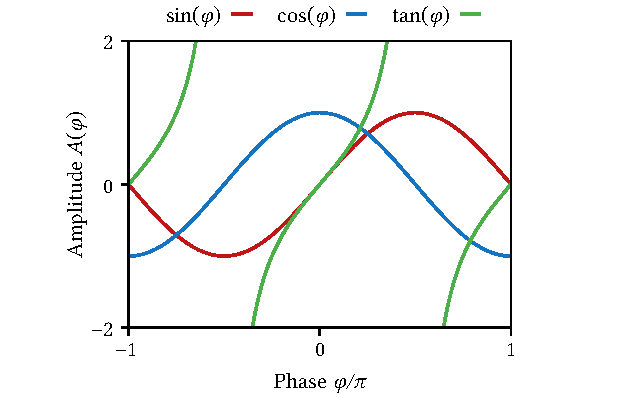
\includegraphics[width=0.2\textwidth]{test.jpg}
  \caption{This is simply a test figure, and some equation $\sin(2x)=1$, and some SI unit \SI{1.0e3}{m/s}, and some chemical \ce{CrO2}. This text can even be made even longer, since we want to test this properly.}
  \label{fig:test}
\end{figure}


Morbi non tortor volutpat, mattis odio at, tincidunt libero.
Donec pulvinar et mi at varius.
Sed vulputate lectus eu libero gravida, vel porta tortor bibendum.
Quisque dictum ex id quam ultrices, ut commodo nisl euismod.
Aliquam vulputate, urna quis sodales rhoncus, orci metus pulvinar velit, feugiat sollicitudin dui massa interdum tortor.
Nam sed ante vitae eros imperdiet bibendum.
Fusce pretium semper leo eget lobortis.
Sed dictum erat quis diam faucibus bibendum.
Integer vitae enim euismod, ornare augue quis, pharetra ante.
Phasellus venenatis tellus ut velit faucibus, posuere porttitor lacus hendrerit.

\begin{table}[h!]
  \centering
  \caption{This is simply a test table.}
  \label{tab:test}
  \begin{tabular*}{\dimexpr\textwidth-4em\relax}{@{\extracolsep{\stretch{1}}\,}lcc@{\,}}
    \toprule
    Name    &   Symbol    &   Value             \\
    \midrule
    Euler constant          & $e$   & $2.71...$  \\
    Circle constant         & $\pi$ & $3.14...$ \\
    Imaginary identity      & $i$ & $\sqrt{-1}$ \\
    \bottomrule
  \end{tabular*}
\end{table}

Lorem ipsum dolor sit amet, consectetur adipiscing elit.
Donec malesuada magna sem.
Fusce vitae lectus id magna convallis euismod.
Quisque viverra sollicitudin turpis, vel ultricies mauris dictum quis.
Praesent justo nunc, luctus in lectus in, placerat tempus orci.
Donec placerat neque ac tortor dignissim pellentesque.
Aenean tellus erat, eleifend id interdum a, volutpat et massa.
Quisque tristique accumsan efficitur.

Morbi non tortor volutpat, mattis odio at, tincidunt libero.
Donec pulvinar et mi at varius.
Sed vulputate lectus eu libero gravida, vel porta tortor bibendum.
Quisque dictum ex id quam ultrices, ut commodo nisl euismod.
Aliquam vulputate, urna quis sodales rhoncus, orci metus pulvinar velit, feugiat sollicitudin dui massa interdum tortor.
Nam sed ante vitae eros imperdiet bibendum.
Fusce pretium semper leo eget lobortis.
Sed dictum erat quis diam faucibus bibendum.
Integer vitae enim euismod, ornare augue quis, pharetra ante.
Phasellus venenatis tellus ut velit faucibus, posuere porttitor lacus hendrerit.

Lorem ipsum dolor sit amet, consectetur adipiscing elit.
Donec malesuada magna sem.
Fusce vitae lectus id magna convallis euismod.
Quisque viverra sollicitudin turpis, vel ultricies mauris dictum quis.
Praesent justo nunc, luctus in lectus in, placerat tempus orci.
Donec placerat neque ac tortor dignissim pellentesque.
Aenean tellus erat, eleifend id interdum a, volutpat et massa.
Quisque tristique accumsan efficitur.


\section{Continuation}
Morbi non tortor volutpat, mattis odio at, tincidunt libero.
Donec pulvinar et mi at varius.
Sed vulputate lectus eu libero gravida, vel porta tortor bibendum.
Quisque dictum ex id quam ultrices, ut commodo nisl euismod.
Aliquam vulputate, urna quis sodales rhoncus, orci metus pulvinar velit, feugiat sollicitudin dui massa interdum tortor.
Nam sed ante vitae eros imperdiet bibendum.
Fusce pretium semper leo eget lobortis.
Sed dictum erat quis diam faucibus bibendum.
Integer vitae enim euismod, ornare augue quis, pharetra ante.
Phasellus venenatis tellus ut velit faucibus, posuere porttitor lacus hendrerit.

Lorem ipsum dolor sit amet, consectetur adipiscing elit.\cite{feynman,statistics}\footnote{test}
Donec malesuada magna sem.
Fusce vitae lectus id magna convallis euismod.
Quisque viverra sollicitudin turpis, vel ultricies mauris dictum quis.
Praesent justo nunc, luctus in lectus in, placerat tempus orci.
Donec placerat neque ac tortor dignissim pellentesque.
Aenean tellus erat, eleifend id interdum a, volutpat et massa.
Quisque tristique accumsan efficitur.

Morbi non tortor volutpat, mattis odio at, tincidunt libero.
Donec pulvinar et mi at varius.
Sed vulputate lectus eu libero gravida, vel porta tortor bibendum.
Quisque dictum ex id quam ultrices, ut commodo nisl euismod.
Aliquam vulputate, urna quis sodales rhoncus, orci metus pulvinar velit, feugiat sollicitudin dui massa interdum tortor.\footnote{This is another footnote test.} %\footnote{This is simply just a simple test, with an equation $\sin \alpha = \cos(2a-1)/\cos(2a+1)$. And here is a chemical element \ce{CrO23} and physical unit \SI{12e3}{m}. }\footnote{Here is another footnote, also set in sans-serif.}%\footnote{$ABCDEFGHIJKLMOPQRSTUVWXYZ$ $abcdefghijklmopqrstuvwxyz$ $\alpha\beta\gamma\delta$ $\Gamma\Delta$ $\int_0^\infty \mathrm{d}x\,\sum_{ij} f(x_{ij}) \leq 0 \mathbf{xyz} \hat{x}+\check{y}\cdot\bar{u} \mathcal{F} \mathbf{x\sigma}$ $\sin x$  $\cos x$}
Nam sed ante vitae eros imperdiet bibendum. 
Fusce pretium semper leo eget lobortis.
Sed dictum erat quis diam faucibus bibendum.
Integer vitae enim euismod, ornare augue quis, pharetra ante.
Phasellus venenatis tellus ut velit faucibus, posuere porttitor lacus hendrerit.

Lorem ipsum dolor sit amet, consectetur adipiscing elit.
Donec malesuada magna sem.
Fusce vitae lectus id magna convallis euismod.
Quisque viverra sollicitudin turpis, vel ultricies mauris dictum quis.
Praesent justo nunc, luctus in lectus in, placerat tempus orci.
Donec placerat neque ac tortor dignissim pellentesque.
Aenean tellus erat, eleifend id interdum a, volutpat et massa.
Quisque tristique accumsan efficitur.

Morbi non tortor volutpat, mattis odio at, tincidunt libero.
Donec pulvinar et mi at varius.
Sed vulputate lectus eu libero gravida, vel porta tortor bibendum.
Quisque dictum ex id quam ultrices, ut commodo nisl euismod.
Aliquam vulputate, urna quis sodales rhoncus, orci metus pulvinar velit, feugiat sollicitudin dui massa interdum tortor.
Nam sed ante vitae eros imperdiet bibendum.
Fusce pretium semper leo eget lobortis.
Sed dictum erat quis diam faucibus bibendum.\footnote{Test}\cite{particle}
Integer vitae enim euismod, ornare augue quis, pharetra ante.
Phasellus venenatis tellus ut velit faucibus, posuere porttitor lacus hendrerit.


%
%\clearpage
%\chapter*{Bestemte integral}\noindent
%Under skal jeg prøve å gi en rask intro til bestemt integrasjon.
%Måten jeg gjør det på, er som følger: jeg kommer bare til å hoppe rett inn i det ved å demonstrere hvordan man løser to eksempeloppgaver.
%Etter det, skal jeg prøve å gi en kort oppsummering av hvordan man logisk kan tenke på bestemte integraler etterpå.
%Dette blir ikke en veldig dyp intro, men håper at det gir deg det du trenger for å løse eksamensoppgavene iallefall :).
%
%\section*{Eksempel I: introduksjon}\noindent
%La oss starte med et relativt enkelt eksempel på et bestemt integral:
%\begin{equation*}
%  \int_{x=0}^{x=1} x^2\,\text{d}x
%\end{equation*}
%Dette skrives ofte uten $x=\cdots$, altså på kortformen:
%\begin{equation*}
%  \int_{0}^{1} x^2\,\text{d}x
%\end{equation*}
%Når man skal løse et bestemt integral, må man alltid starte med å løse det ubestemte integralet.
%Hvis du slår opp i formelsamlingen bakerst i et av eksamenssettene, finner du en formel for ubestemte integral av polynomer:
%\begin{align*}
%  \int x^r\;\text{d}x &= \frac{1}{r+1} x^{r+1} & &\text{(for $r\neq-1$)}
%\end{align*}
%Setter du inn $r=2$ finner du da:
%\begin{align*}
%  \int x^2\;\text{d}x = \frac{1}{3} x^3
%\end{align*}
%Okay, la oss nå gå tilbake til det \emph{bestemte} integralet.
%Den vanlige måten å skrive ned at man har løst det \emph{ubestemte} integralet på, er å sette firkantklammer rundt svaret, med de såkallte \emph{integrasjonsgrensene} 0 og 1 utenfor klammene:
%\begin{equation*}
%  \int_{x=0}^{x=1} x^2\,\text{d}x = \left[ \frac{1}{3} x^3 \right]_{x=0}^{x=1}
%\end{equation*}
%Det å faktisk regne ut det bestemte integralet fra det ubestemte er nå veldig enkelt: vi trenger faktisk bare å sette inn $x=1$ og $x=0$ i det uttrykket som står i klammer, og så trekke svarene fra hverandre:
%\begin{align*}
%  \left[ \frac{1}{3} x^3 \right]_{x=0}^{x=1} 
%  &= \left[ \frac{1}{3} x^3 \right]_{x=1} - \;\;\;\;\left[ \frac{1}{3} x^3 \right]_{x=0} \\
%  &= \left[ \frac{1}{3} \cdot 1^3 \right]\;\;\; - \;\;\;\left[ \frac{1}{3} \cdot 0^3 \right] \\
%  &= \frac{1}{3} - 0 \\
%  &= \frac{1}{3}
%\end{align*}
%Svaret fra den bestemte integrasjonen blir altså:
%\begin{equation*}
%  \int_0^1 x^2\,\text{d}x = \frac{1}{3}
%\end{equation*}
%
%\section*{Eksempel II: avansert}
%Okay, la oss se på en litt mer avansert oppgave:
%\begin{equation*}
%  \int_1^\infty e^{-2x}
%\end{equation*}
%Første steg er som sagt alltid å løse det ubestemte integralet. 
%Sjekker du formelsamlingen bakerst i et eksamenssett dine, finner du denne likningen:
%\begin{align*}
%  \int e^{kx}\;\text{d}x &= \frac{1}{k} e^{kx} + C & &\text{($C$ er en vilkårlig konstant)}
%\end{align*}
%Sett inn at $k=-2$:
%\begin{align*}
%  \int e^{-2x}\;\text{d}x &= -\frac{1}{2} e^{-2x} + C
%\end{align*}
%Så løsningen på det ubestemte integralet er også:
%\begin{align*}
%  \int_{1}^{\infty} e^{-2x}\;\text{d}x &= \left[ -\frac{1}{2} e^{-2x} + C \right]_1^\infty
%\end{align*}
%Vi finner da løsningen på det bestemte integralet ved å sette inn $x=\infty$ og $x=1$, og trekke resultatene fra hverandre.
%En detalj som trengs her, er da at $e^{-\infty} = 1/e^{\infty} = 1/\infty = 0$; har du ikke lært om grenseverdier i faget, så trenger du ikke å tenke så mye på dette, det er isåfall muligens utenfor pensum :).
%Men beregningen blir altså:
%\begin{align*}
%  \int_{1}^{\infty} e^{-2x}\;\text{d}x 
%  &= \left[ -\frac{1}{2} e^{-2x}     + C \right]_1^\infty \\
%  &= \left[ -\frac{1}{2} e^{-2x}     + C \right]_{x=\infty} - \;\;\;\;\left[ -\frac{1}{2} e^{-2x} + C \right]_{x=1} \\
%  &= \left[ -\frac{1}{2} e^{-\infty} + C \right] \;\;\;\;\;\; - \;\;\;\; \left[ -\frac{1}{2} e^{-2} + C \right] \\
%  &= \left[ -\frac{1}{2} \cdot 0 \; +  C \right] \;\;\;\;\;\; - \;\;\;\; \left[ -\frac{1}{2} e^{-2} + C \right] \\
%  &= 0 + C + \frac{1}{2} e^{-2} - C \\
%  &= \frac{1}{2} e^{-2} \\
%  &= \frac{1}{2e^2}
%\end{align*}
%Så svaret er:
%\begin{align*}
%  \int_{1}^{\infty} e^{-2x}\;\text{d}x &= \frac{1}{2e^2}
%\end{align*}
%Merk at det ikke hadde noe å si at vi ikke visste hva den ukjente konstanten $C$ var for noe, den forsvant uansett når vi beregnet et bestemt integral :).
%
%\section*{Tolkning I: antiderivasjon}
%En måte å tolke hva integrasjon betyr for noe, er at det er \emph{det omvendte av derivasjon}. 
%For eksempel, hvis vi tar det ubestemte integralet vi så på over:
%\begin{align*}
%  \int x^2\;\text{d}x &= \frac{1}{3} x^{3}
%\end{align*}
%Hva skjer hvis vi deriverer svaret? 
%Jo, den deriverte av $x^{3}$ er $3x^2$, så vi får:
%\begin{align*}
%  \left( \int x^2\;\text{d}x \right)' &= x^{2}
%\end{align*}
%Så hvis vi først integrerer $x^2$ og så deriverer svaret, så får vi tilbake det vi startet med.
%Derivasjonen gjorde det motsatte av det integrasjonen gjorde.
%
%Hva betyr dette for hvordan vi skal tolke integrasjon?
%Jo, det derivasjon måler er jo \emph{stigningstallet} eller \emph{endringsraten} til noe.
%For eksempel, hvis du vet posisjonen $s$ til en bil som funksjon av tiden $t$, så vil den deriverte $v(t) = s'(t)$ være \emph{hastigheten} til bilen.
%Siden integrasjon gjør det motsatte, betyr det at du kan integrere hastigheten for å finne ut hvor langt bilen faktisk har kjørt.
%
%
%\section*{Tolkning II: areal under en kurve}
%En geometrisk tolkning av integrasjon, er at det er en måte å regne ut arealet under en kurve.
%La oss f.eks. si at vi har en graf av funksjonen $f(x) = 1-x^2$:\\
%{\quad \includegraphics[width=0.6\textwidth]{/home/jabirali/figure.png}} \\
%Hvis vi tar et bestemt integral av denne funksjonen fra $x=0$ til $x=1$:
%\begin{equation*}
%  \int_0^1 (1-x^2)\;\text{d}x = \left[ x - \frac{1}{3}x^3 \right]_0^1 = [1 - 1/3] - [0 - 0] = 2/3
%\end{equation}
%Egentlig bare arealet under kurven mellom $x=0$ og $x=1$:\\
%{\quad \includegraphics[width=0.6\textwidth]{/home/jabirali/areal.png}}\\
%Det å \emph{bevise} at integraler gir deg areal er litt mer jobb, og sannsynligvis ikke verdt å fokusere på fram mot eksamen.
%Men det er greit å ha i bakhodet at hvis det kommer en eksamensoppgave hvor de vil at du skal ``finne arealet under kurven'', så betyr det bare at du skal løse et bestemt integral ;).
%
%Det at ``integral'' betyr ``areal under kurve'' gir jo en innsikt til.
%Et ``bestemt integral fra $x=0$ til $x=1$'' er altså arealet under kurven mellom punktene $x=0$ og $x=1$.
%Et ``ubestemt integral'' derimot, hvor vi ikke har satt inn noen verdier for $x$ enda, er en generell formel for å regne ut arealet under kurven for vilkårlige startpunkt og sluttpunkt.
%Dette minner jo litt om den samme situasjonen for derivasjon: $f'(x)$ er en ``ubestemt derivert'', altså en generell formel for å regne ut stigningstall. Hvis du setter inn $x=2$ i dette uttrykket, altså beregner $f'(2)$, så har du derimot spesifikt stigningstallet til kurven i punktet $x=2$, som vi godt kunne kallt en ``bestemt derivert''.






\backmatter
\printbibliography

\end{document}
